\documentclass[10pt,landscape,a4paper]{article}
\usepackage{multicol}
\usepackage{calc}
\usepackage{ amssymb }
\usepackage{ifthen}
\usepackage[landscape]{geometry}
\usepackage{amsmath,amsthm,amsfonts}%,amssymb}
\usepackage{color,graphicx,overpic}
\usepackage{hyperref}
\usepackage{braket}
\usepackage{pdfpages}


% This sets page margins to .5 inch if using letter paper, and to 1cm
% if using A4 paper. (This probably isn't strictly necessary.)
% If using another size paper, use default 1cm margins.
\ifthenelse{\lengthtest { \paperwidth = 11in}}
    { \geometry{top=.5in,left=.5in,right=.5in,bottom=.5in} }
    {\ifthenelse{ \lengthtest{ \paperwidth = 297mm}}
        {\geometry{top=1cm,left=1cm,right=1cm,bottom=1cm} }
        {\geometry{top=1cm,left=1cm,right=1cm,bottom=1cm} }
    }
\newcommand{\RSr}{\frac{2GM}{r}}
\newcommand{\intgr} {\mathrm{d}}

\newcommand{\metr}{g_{\mu\nu}}
\newcommand{\metrup}{g^{\mu\nu}}
\newcommand{\half}{\frac{1}{2}}
\newcommand{\munu} {\mu\nu}

\newcommand{\der}[2] {\frac{d #1}{d #2}}
\newcommand{\dder}[2] {\frac{d^2 #1}{d #2^2}}
\newcommand{\pd}[2] {\frac{\partial #1}{\partial #2}}
\renewcommand{\div}[1] {\nabla\cdot\vec{#1}}
\newcommand{\curl}[1] {\nabla\times\vec{#1}}
\newcommand{\e}[1] {\times 10^{#1}}
\newcommand{\mean}[1] {\langle #1 \rangle}
\newcommand{\expect}[3]{\langle #1 | #2 | #3 \rangle}
\newcommand{\intfy}{\int_{-\infty}^{\infty}}
\newcommand{\intzfy}{\int_0^\infty}
\newcommand{\centerthis}[1]{\makebox[\textwidth]{#1}}

% Turn off header and footer
\pagestyle{empty}

% Redefine section commands to use less space
\makeatletter
\renewcommand{\section}{\@startsection{section}{1}{0mm}%
                                {-1ex plus -.5ex minus -.2ex}%
                                {0.5ex plus .2ex}%x
                                {\normalfont\large\bfseries}}
\renewcommand{\subsection}{\@startsection{subsection}{2}{0mm}%
                                {-1explus -.5ex minus -.2ex}%
                                {0.5ex plus .2ex}%
                                {\normalfont\normalsize\bfseries}}
\renewcommand{\subsubsection}{\@startsection{subsubsection}{3}{0mm}%
                                {-1ex plus -.5ex minus -.2ex}%
                                {1ex plus .2ex}%
                                {\normalfont\small\bfseries}}
\makeatother

% Define BibTeX command
\def\BibTeX{{\rm B\kern-.05em{\sc i\kern-.025em b}\kern-.08em
    T\kern-.1667em\lower.7ex\hbox{E}\kern-.125emX}}

% Don't print section numbers
\setcounter{secnumdepth}{0}


\setlength{\parindent}{0pt}
\setlength{\parskip}{0pt plus 0.5ex}

%My Environments
\newtheorem{example}[section]{Example}
% -----------------------------------------------------------------------

\begin{document}
\raggedright
\footnotesize
\begin{multicols}{3}

\setlength{\premulticols}{1pt}
\setlength{\postmulticols}{1pt}
\setlength{\multicolsep}{1pt}
\setlength{\columnsep}{2pt}


\section{Line element}
\begin{equation}
\mathrm{d}s^2 = g_{\munu}\mathrm{d}x^\mu\mathrm{d}x^\nu = -\mathrm{d}\tau^2
\end{equation}
\section{Geodesic equation}
\begin{equation}
\frac{\mathrm{d}^2 x^\mu}{\mathrm{d}\lambda^2} +\Gamma^\mu_{\rho\sigma}\frac{\mathrm{d} x^\rho}{\mathrm{d}\lambda}\frac{\mathrm{d} x^\sigma}{\mathrm{d}\lambda} = 0
\end{equation}

\section{Lorentz transformations}
Rotation x-y plane (around z)
\begin{equation}
\Lambda^{\mu^\prime}_\nu =   
\begin{pmatrix}    1 & 0 & 0 & 0 \\ 0 & \cos\theta & \sin\theta & 0 \\ 
0 & -\sin\theta &\cos\theta & 0 \\ 0 & 0 & 0 & 1
\end{pmatrix}
\end{equation}
Boost x-direction
\begin{equation}
\Lambda^{\mu^\prime}_\nu =   
\begin{pmatrix}    \gamma & \gamma v & 0 & 0 \\ \gamma v & \gamma & 0 & 0 \\ 
0 & 0 & 1 & 0 \\ 0 & 0 & 0 & 1
\end{pmatrix}
\end{equation}

\section{Tensors}
For any two indices we can decompose a tensor into symmetric and anti-symmetric parts
\begin{equation}
T_{\mu\nu\sigma\rho} = T_{(\mu\nu)\sigma\rho} + T_{[\mu\nu]\sigma\rho}
\end{equation}

\section{Levi-Civita}
\begin{equation}
\epsilon_{\mu\nu\sigma\rho} = 
\begin{cases}
+1  &\text{if } \mu\nu\sigma\rho \text{ even permutation of 0123}\\
-1  &\text{if } \mu\nu\sigma\rho \text{  odd permutation of 0123}\\
0   & \text{otherwise}
\end{cases}
\end{equation}
\section{Einstein Equation}
\begin{equation}
R_{\munu} -\frac{1}{2}Rg_{\munu} = 8\pi G T_{\munu} = G_{\munu}
\end{equation}
With vacuum energy
\begin{equation}
R_{\munu} -\frac{1}{2}Rg_{\munu} + \Lambda g_{\munu} = 8\pi G T_{\munu}
\end{equation}
\begin{equation}
\nabla^\mu G_{\munu} = 0
\end{equation}
Can also write 
\begin{equation}
R_{\munu} = 8\pi G(T_{\munu} -\frac{1}{2}Tg_{\munu})
\end{equation}
\section{Schwarzschild metric}
\begin{equation}
\mathrm{d}s^2 = -(1+R_s/r)\mathrm{d}t^2 + (1+R_s/r)^{-1}\mathrm{d}r^2 + r^2\mathrm{d}\Omega^2,
\end{equation}
where $\mathrm{d}\Omega^2 = (\mathrm{d}\theta^2+ \sin^2\theta \mathrm{d}\phi^2)$

\section{Eddington-Finkelstein coordinates}
\begin{equation}
\mathrm{d}s^2 = -(1-\frac{2GM}{r})\mathrm{d}v^2 + (\intgr v \intgr r + \intgr r \intgr v) +r^2 \intgr\Omega^2
\end{equation}
\begin{equation}
v = t+ r^\star, u =t-r^\star
\end{equation}
\begin{equation}
r^\star = r +2GM\ln(\frac{r}{2GM}-1)
\end{equation}
Infalling radial null geodesics characterized by $v=\text{const}$, and utgoing ones by $u=\text{const}$.

\section{Kruskal coordinates}
\begin{equation}
\intgr s^2 = \frac{32G^3M^3}{r} e^{-r/2GM}(-\intgr T^2 + \intgr R^2) +r^2 \intgr\Omega^2
\end{equation}
\begin{equation}
T^2-R^2=(1-\frac{r}{2GM})e^{r/2GM}
\end{equation}
Radial null curves have 
\begin{equation}
T = \pm R+ \text{const}
\end{equation}
Event horizon at 
\begin{equation}
T = \pm R
\end{equation}
Surfaces with constant $r$ have
\begin{equation}
T^2-R^2 = \text{const}
\end{equation}
while surfaces of constant $t$ have
\begin{equation}
\frac{T}{R} = \tanh(\frac{t}{4GM})
\end{equation}

\section{Penrose/Kruskal diagrams}
Schwarzschild
\begin{minipage}{0.9\linewidth}
\centering
    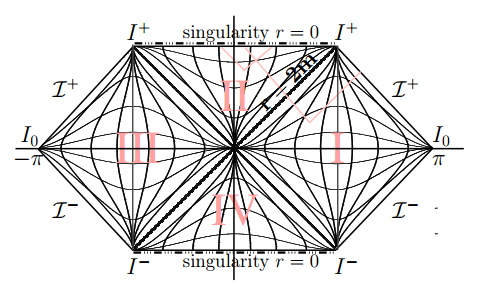
\includegraphics[width=\linewidth]{penrose-kruskal.png}
    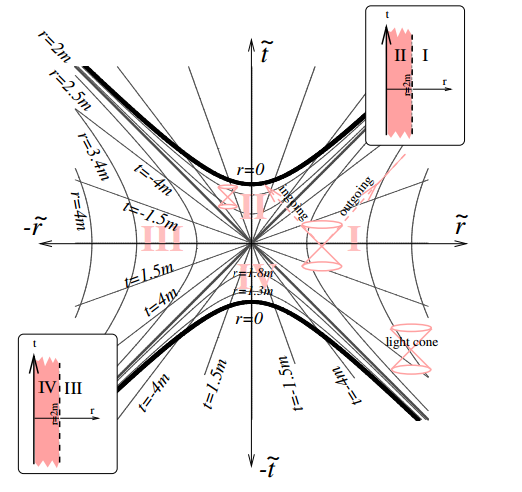
\includegraphics[width=\linewidth]{kruskal.png}
\end{minipage}

Kerr

\begin{minipage}{0.9\linewidth}
\centering
    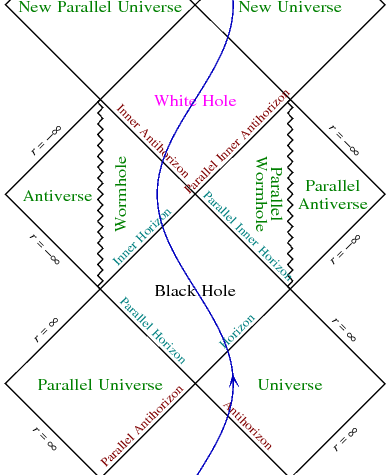
\includegraphics[width=\linewidth]{kerr.png}
\end{minipage}

\section{Thermodynamics}
First law of thermodynamics
\begin{equation}
\intgr E = T \intgr S - p \intgr V
\end{equation}
For black holes $E \leftrightarrow M$, $S \leftrightarrow A/4G$, $T \leftrightarrow \kappa/2\pi$.

\section{Killing vectors}
Killing's equation
\begin{equation}
\nabla_{(\mu}K_{\nu)} = 0 \Rightarrow p^\mu\nabla_\mu(K_\nu p^\nu) = 0
\end{equation}
If the metric is independent of time we know that $K^\mu=(1,0,0,0)$ is a killing vector. We also know that $K_\mu$ will satisfy Killings equation, which after some manipulation turns into
\begin{equation}
K_\mu U^\mu = \mathrm{const},
\end{equation}
where $U^\mu$ is the four-velocity. 

E.g in Schwarzschild:
Metric is indep. of $t$ and $\phi$ so $K^\mu$ is a killing vector.
\begin{equation}
K_\mu = g_{\mu\nu}K^\nu = (-(1+R_s/r),0,0,0),
\end{equation}
\begin{equation}
R_\mu = g_{\mu\nu}R^\nu = (0,0,0,r^2\sin^2\theta)
\end{equation}
which leads to 
\begin{equation}
K_\mu U^\mu = -(1+R_s/r)\mathrm{d}t^2/\mathrm{d}\tau^2 = -E
\end{equation}
\begin{equation}
R_\mu U^\mu = r^2\sin^2\theta\mathrm{d}\phi^2/\mathrm{d}\tau^2 = L
\end{equation}


\section{Geodesic deviation}
\begin{equation}
A^\mu =\frac{D^2}{\mathrm{d}t^2}S^\mu = R^\mu_{\nu\rho\sigma}T^\nu T^\rho S^\sigma
\end{equation}

\section{Metric of a star}
\begin{equation}
\intgr s^2 = -e^{2\alpha(r)}\intgr t^2 +e^{2\beta(r)}\intgr r^2 +r^2\intgr\Omega^2
\end{equation}
where $\Omega^2 = (\mathrm{d}\theta+ \sin^2\theta \mathrm{d}\phi^2)$, and
\begin{equation}
e^{2\beta(r)} = \bigg(1-\frac{2GM}{r}\bigg)^{-1},
\end{equation}
and
\begin{equation}
e^{2\alpha(r)} = \frac{3}{2}\bigg(1-\frac{2GM}{R}\bigg)^{1/2} -\frac{1}{2}\bigg(1-\frac{2GMr^2}{R^3}\bigg)^{1/2}, r< R
\end{equation}

\section{Charged BH}
Formally known as Reissner-Nordström black holes.
\begin{equation}
\intgr s^2 = -\Delta \intgr t^2 +\Delta^{-1} \intgr r^2 + r^2 \intgr\Omega^2
\end{equation}
with 
\begin{equation}
\Delta = 1-\frac{2GM}{r} + \frac{G(Q^2+P^2)}{r^2}.
\end{equation}
Q is the electric charge, and P the total magnetic charge.
This is a black hole and magnetic monopoles have not been observed, so usually we set $P = 0$.
\begin{equation}
E_r = F_{rt} = \frac{Q}{r^2}
\end{equation}
\begin{equation}
B_r = \frac{F_{\theta\phi}}{r^2\sin\theta} = \frac{P}{r^2}
\end{equation}
Event horizon located at
\begin{equation}
r_\pm = GM \pm \sqrt{G^2M^2-G(Q^2+P^2)}
\end{equation}

\section{Rotating BH}
Formally known as Kerr black holes.
\begin{equation}
\begin{split}
\intgr s^2 = -(1-\frac{2GM}{\rho^2})\intgr t^2 - \frac{2GMar\sin^2\theta}{\rho^2}(\intgr t \intgr \phi + 
\intgr\phi\intgr t) \\ + \frac{\rho^2}{\Delta}\intgr r^2 +  
\rho^2 \intgr\theta^2 +\frac{\sin^2\theta}{\rho^2}[(r^2 + a^2)^2 - 
a^2\Delta\sin^2\theta]\intgr\phi^2,\\
\end{split}
\end{equation}
\begin{equation}
\Delta(r) = r^2 - 2GMr + a^2,
\end{equation}
\begin{equation}
\rho^2(r,\theta) = r^2 + a^2 \cos\theta.
\end{equation}
Where $a=J/M$ is the angular momentum per mass,
where J is the Komar angular momentum. 
\section{Equivalence principle}
\subsection{Weak}
The trajectory of a point mass in a gravitational field depends only on its initial position and velocity, and is independent of its composition and structure.

All test particles at the alike spacetime point, in a given gravitational field, will undergo the same acceleration, independent of their properties, including their rest mass.

All local centers of mass free-fall (in vacuum), along identical (parallel-displaced, same speed) minimum action trajectories independent of all observable properties.

The vacuum world-line of a body immersed in a gravitational field is independent of all observable properties.

The local effects of motion in a curved spacetime (gravitation) are indistinguishable from those of an accelerated observer in flat spacetime, without exception.

Mass (measured with a balance) and weight (measured with a scale) are locally in identical ratio for all bodies (the opening page to Newton's Philosophiæ Naturalis Principia Mathematica, 1687).
\subsubsection{Tests}
Tests that check whether gravitational mass and inertial mass are the same.
See for example Schlamminger, Stephan, et al. "Test of the equivalence principle using a rotating torsion balance." Physical Review Letters 100.4 (2008): 041101. The conclusion is that the violation is extremely small if it exists at all. At the moment 
\subsection{Einstein}
The weak equivalence principle holds and

The outcome of any local non-gravitational experiment in a freely falling laboratory is independent of the velocity of the laboratory and its location in spacetime.
By local one means that one can not look outside the laboratory and the laboratory must be small compared to variations in the gravitational field. This also means that no other fields than gravity can be nearby.

\subsubsection{Tests}
In addition to the tests of the weak equivalence principle, the Einstein equivalence principle can be tested by searching for variation of dimensionless constants and mass ratios. 
Examples of experiments conducted to test this include measurements of the fine structure constant using quasars, and gravitational redshift	experiments where the position independence is tested.

\subsection{Strong}
The strong equivalence principle suggests the laws of gravitation are independent of velocity and location. In particular,

The gravitational motion of a small test body depends only on its initial position in spacetime and velocity, and not on its constitution.

The outcome of any local experiment (gravitational or not) in a freely falling laboratory is independent of the velocity of the laboratory and its location in spacetime.

This requires the gravitational constant to be the same everywhere.
In short this allows for self gravitating bodies. It also means that gravity is entirely geometric by nature meaning that if one finds a piece of space to be flat, it is exactly the same as any other piece of flat space regardless of their positions.

General Relativity is the only theory known today that satisfies the strong equivalence principle.
There are other theory that only satisfy the Einstein equivalence principle such as Brans-Dicke theory.

\subsubsection{Tests}
To test the strong equivalence principle we measure variations in the gravitational constant G throughout the life of the universe.
One can also look for fifth forces at large distances. Typically extrasolar scales and up. 
To test it in the lab one can look for failures of the inverse square law. 

\section{Experimental tests}
See tests of equivalence principle.
Einstein suggested three test: the deflection of light, the precession of perihelia, and gravitational redshift. Measurements of the precession of mercury was the first major confirmation of GR being correct.

\section{Weak limit}
\begin{equation}
\mathrm{d}s^2 = -(1+\phi)\mathrm{d}t^2 + (1-\phi)\delta^i_j\mathrm{d}x^i\mathrm{d}x^j,
\end{equation}
with
\begin{equation}
\phi = -GM/\sqrt{x^2+y^2+z^2}
\end{equation}
\section{Differential geometry}
\begin{equation}
\nabla_\mu V^\nu = \partial_\mu V^\nu + \Gamma^\nu_{\mu\lambda}V^\lambda
\end{equation}
\begin{equation}
\nabla_\mu V_\nu = \partial_\mu V_\nu - \Gamma^\lambda_{\mu\nu} V_\lambda
\end{equation}
You add a + for each upper and a - for each lower. Like so
\begin{equation}
\nabla_\mu T^\nu_\rho = \partial_\mu T^\nu_\rho + \Gamma^\nu_{\mu\lambda}T^\lambda_\rho - \Gamma^\lambda_{\mu\rho}T^\nu_\lambda
\end{equation}

\section{Einstein Hilbert action}
\begin{equation}
S_H = \int \sqrt{-g}R d^n x
\end{equation}
Can't plug into Lagrange equations so we vary with respect to the inverse metric instead.
\begin{equation}
\delta g_{\munu} = -g_{\mu\rho}g_{\nu\sigma}\delta g^{\rho\sigma}, R = g^{\munu}R_{\munu}
\end{equation}
\begin{equation}
delta S_H = (\delta S)_1 + (\delta S)_2 + (\delta S)_3,
\end{equation}
where
\begin{equation}
(\delta S)_1 = \int d^n \sqrt{-g}g^{\munu}\delta R_{\munu}
\end{equation}
\begin{equation}
(\delta S)_2 = \int d^n \sqrt{-g}R_{\munu}\delta g^{\munu}
\end{equation}
\begin{equation}
(\delta S)_3 = \int d^n R\delta \sqrt{-g}
\end{equation}
This approach eventually leads to the einstein equation.

One can include matter by writing
\begin{equation}
S = \frac{1}{16\pi G} S_H + S_M
\end{equation}
which leads to 
\begin{equation}
T_{\munu} = -2\frac{1}{\sqrt{-g}}\frac{\delta S_M}{\delta g^{\munu}}
\end{equation}

\section{Weyl tensor}
\begin{equation}
C_{\rho\sigma\munu} = R_{\rho\sigma\munu}+\frac{1}{3}g_{\rho[\mu}g_{\nu]\sigma}R-g_{\rho[\mu}R_{\nu]\sigma} + g_{\sigma[\mu}R_{\nu]\rho}
\end{equation}
\section{Christoffel symbols}
\begin{equation}
\Gamma^\lambda_{\munu} = \frac{1}{2}g^{\lambda\sigma}(\partial_\mu g_{\nu\sigma} + \partial_\nu g_{\sigma\mu} -\partial_\sigma g_{\munu})
\end{equation}
\section{Lagrange}
Lagrange's equation
\begin{equation}
\frac{\mathrm{d}}{\mathrm{d}t}\bigg(\frac{\partial L}{\partial(\dot{q})}\bigg) - \frac{\partial L}{\partial q} = 0
\end{equation}

\section{Riemann/Ricci tensor/scalar}
Riemann tensor
\begin{equation}
R^\rho{}_{\sigma\munu} = 
 \partial_\mu \Gamma^\rho_{\nu\sigma}
-\partial_\nu \Gamma^\rho_{\mu\sigma}
+\Gamma^\rho_{\mu\lambda}\Gamma^\lambda_{\nu\sigma} 
-\Gamma^\rho_{\nu\lambda}\Gamma^\lambda_{\mu\sigma}
\end{equation}
Symmetric in first two indices
\begin{equation}
R_{\rho\sigma\munu} = R_{\sigma\rho\munu}
\end{equation}
Anti-symmetric in last two indices
\begin{equation}
R_{\rho\sigma\munu} = R_{\rho\sigma\nu\mu}
\end{equation}
\begin{equation}
R^\rho{}_{\sigma\munu} = -R^\rho{}_{\sigma\nu\mu}
\end{equation}
Invariant under interchange of two first with two last
\begin{equation}
R_{\rho\sigma\munu} = R_{\nu\mu\rho\sigma}
\end{equation}
Which also means that
\begin{equation}
R_{\rho\sigma\munu} + R_{\rho\mu\nu\sigma} + R_{\rho\nu\sigma\mu} = 0
\end{equation}
and
\begin{equation}
R_{\rho[\sigma\munu]} = 0
\end{equation}

Ricci tensor
\begin{equation}
R_{\munu} = R^\lambda{}_{\mu\lambda\nu}
\end{equation}
Symmetric
\begin{equation}
R_{\munu} = R_{\nu\mu}
\end{equation}
Ricci scalar
\begin{equation}
R = R^\mu{}_{\mu} = g^{\munu}R_{\munu}
\end{equation}
\begin{equation}
\begin{split}
G_{\munu} = R_{\munu}-\frac{1}{2}\eta_{\munu} R\\
= \frac{1}{2}(\partial_\sigma\partial_\nu h^\sigma{}_\mu + \partial_\sigma\partial_\mu h^\sigma{}_\nu -  \partial_\mu\partial_\nu h - \\
\Box h_{\munu} - \eta_{\munu}\partial_\sigma\partial_\lambda h^{\rho\lambda} + \eta_{\munu}\Box h)
\end{split}
\end{equation}
\section{Four velocity/momentum}
\begin{equation}
U^\mu = \frac{\mathrm{d}x^\mu}{\mathrm{d}\tau}
\end{equation}
\begin{equation}
p^\mu = mU^\mu
\end{equation}
\section{Energy momentum tensor}
Perfect fluid
\begin{equation}
T^{\munu} = (\rho+p)U^\mu U^\nu + p\eta^{\munu}
\end{equation}
at rest
\begin{equation}
T^{\munu} = 
\begin{pmatrix} 
\rho &0&0&0\\ 
0&p&0&0\\ 
0&0&p&0\\ 
0&0&0&p 
\end{pmatrix}
\end{equation}

\begin{equation}
\partial_\mu T^{\munu} = 0
\end{equation}

\section{Linearized gravity}
\begin{equation}
g_{\munu} = \eta_{\munu} + h_{\munu} , |h_{\munu}| \ll 1,
\end{equation}
\begin{equation}
g^{\munu} = \eta^{\munu} - h^{\munu} ,
\end{equation}
\begin{equation}
\Gamma^\rho_{\munu} = \frac{1}{2}\eta^{\rho\lambda}(\partial_\mu h_{\nu\lambda} + \partial_\nu h_{\lambda\mu} + \partial_\lambda h_{\munu}),
\end{equation}
\begin{equation}
R_{\mu\nu\rho\sigma} = \frac{1}{2}(\partial_\rho\partial_\nu h_{\mu\sigma} + \partial_\sigma\partial_\mu h_{\nu\rho} -\partial_\sigma\partial_\nu h_{\mu\rho} - \partial_\rho\partial_\mu h_{\nu\sigma}),
\end{equation}
\begin{equation}
R_{\munu} = \frac{1}{2}(\partial_\sigma\partial_\nu h^\sigma_\mu + \partial_\sigma\partial_\mu h^\sigma_\nu - \partial_\mu\partial_\nu h - \Box h_{\munu}),
\end{equation}
\begin{equation}
R = \partial_\mu\partial_\nu h^{\munu} - \Box h,
\end{equation}
where $h = \eta^{\munu}h_{\munu} = h^\mu{}_\mu$, and $\Box = -\partial_t^2+\partial_x^2 +\partial_y^2 + \partial_z^2$.
Can also get to the same Einstein tensor $G_{\munu}$ by varying the following Lagrangian with respect to $h_{\munu}$.
\begin{equation}
\begin{split}
\mathcal{L} = \frac{1}{2}(\partial_\mu h^{\munu})(\partial_\nu h) -(\partial_\mu h^{\rho\sigma})
(\partial_\rho h^\mu_\sigma) \\
+\frac{1}{2}\eta^{\munu}(\partial_\mu h^{\rho\sigma})(\partial_\nu h_{\rho\sigma}) -\frac{1}{2}\eta^{\munu}(\partial_\mu h)(\partial_\nu h)
\end{split}
\end{equation}
Can rewrite the metric into 
\begin{equation}
\begin{split}
h_{00} &= -2\Phi\\
h_{0i} &= w_i\\
h_{ij} &= 2s_{ij} -2\Psi\delta_{ij}.\\
\end{split}
\end{equation}
where $\Psi$ encodes the trace of $h_{ij}$, and $s_{ij}$ is traceless:
\begin{equation}
\begin{split}
\Psi &= \frac{1}{6}\delta^{ij} h_{ij} \\
s_{ij} &= \frac{1}{2}\bigg(h_{ij} - \frac{1}{3}\delta^{kl} h_{kl} \delta_{ij}\bigg) \\
\end{split}
\end{equation}
This leads to 
\begin{equation}
\intgr s^2 = -(1+2\Phi)\intgr t^2 + w_i(\intgr t\intgr x^i +\intgr x^i\intgr t) + [(1-2\Psi)\delta_{ij} + 2s_{ij}]\intgr x^i\intgr x^j
\end{equation}
This has Christoffel symbols
\begin{equation}
\begin{split}
\Gamma^0_{00} &=\partial_0\Phi\\
\Gamma^i_{00} &=\partial_i\Phi +\partial_0 w_i\\
\Gamma^0_{j0} &=\partial_j\Phi\\
\Gamma^i_{j0} &=\partial_{[j}w_{i]} +\frac{1}{2}\partial_0h_{ij}\\
\Gamma^0_{jk} &=-\partial_{(j}w_{k)} +\frac{1}{2}\partial_0h_{jk}\\
\Gamma^i_{jk} &=\partial_{(j}h_{k)i} -\frac{1}{2}\partial_ih_{jk}.\\
\end{split}
\end{equation}
Giving the following Riemann tensor components
\begin{equation}
\begin{split}
R_{0j0l} &= \partial_j\partial_l\Phi +\partial_0\partial_{(j}w_{l)} -\frac{1}{2}\partial_0\partial_0 h_{jl}\\
R_{0jkl} &= \partial_j\partial_{[k}w_{l]} -\partial_0\partial_{[k}h_{l]j}\\
R_{ijkl} &= \partial_j\partial_{[k} h_{l]i} -\partial_i\partial_{[k}h_{l]j}\\
\end{split}
\end{equation}
with Rici tensor
\begin{equation}
\begin{split}
R_{00} &= \nabla^2\Phi +\partial_0\partial_kw^k +3\partial_0^2\Phi \\
R_{0j} &= -\frac{1}{2}\nabla^2w_j +\frac{1}{2}\partial_j\partial_kw^k +2\partial_0\partial_j\Psi +\partial_0\partial_ks_j{}^k  \\
R_{ij} &= -\partial_i\partial_j(\Phi-\Psi)-\partial_0\partial_{(i}w_{j)} +\Box\Psi\delta_{ij} -\Box s_{ij} +2\partial_k\partial_{(i}s_{j)}{}^k \\
\end{split}
\end{equation}
where $\nabla^2 = \delta^{ij}\partial_i\partial_j$ is the three dimensional flat Laplacian.
Finally, the Einstein tensor is
\begin{equation}
\begin{split}
G_{00} &= 2\nabla^2\Psi +\partial_k\partial_l s^{kl}   \\
G_{0j} &= -\frac{1}{2}\nabla^2w_j +\frac{1}{2}\partial_j\partial_kw^k + 2\partial_0\partial_j\Psi+\partial_0\partial_ks_j{}^k   \\
G_{ij} &=  (\delta_{ij}\nabla^2 -\partial_i\partial_j)(\Phi-\Psi) +\delta_{ij}\partial_0\partial_kw^k-\partial_0\partial_{(i}w_{j)}  \\
&+2\delta_{ij}\partial_0^2\Psi -\Box s_{ij} +2\partial_k\partial_{(i}s_{j)}{}^k-\delta_{ij}\partial_k\partial_ls^{kl}.\\
\end{split}
\end{equation}
\section{Newtonian fields and photon trajectories}
Work in restframe with dust giving
\begin{equation}
T_{\munu} = \rho U_\mu U_\nu = \begin{pmatrix}
\rho &&&\\
&0&&\\
&&0&\\
&&&0\\
\end{pmatrix}.
\end{equation}
Sine static we drop all time derivatives, plug into energy momentum tensor and get
\begin{equation}
\begin{split}
\nabla^2\Psi  &=4\pi G\rho\\
\nabla^2w_j &= 0\\
(\delta_{ij}\nabla^2 -\partial_i\partial_j)(\Phi -\Psi) -\nabla^2 s_{ij} &= 0\\
\end{split}
\end{equation}
Trace of last
\begin{equation}
2\nabla^2(\Phi-\Psi) = 0
\end{equation}
So $\Phi=\Psi$. Plug this into equations above and get
\begin{equation}
\nabla^2 s_{ij} = 0
\end{equation}
meaning $s_ij = 0$.

The perturbed metric for the static Newtonian source is thus
\begin{equation}
\intgr s^2 = -(1+2\Phi)\intgr t^2 + (1-2\Phi)(\intgr x^2 +\intgr y^2 +\intgr z^2)
\end{equation}
or if you want
\begin{equation}
h_{\munu} = \begin{pmatrix}
-2\Phi&&&\\
&-2\Phi&&\\
&&-2\Phi&\\
&&&-2\Phi\\
\end{pmatrix}
\end{equation}
where the potential obeys the conventional Poisson equation
\begin{equation}
\nabla^2 \Phi = 4\pi G\rho
\end{equation}
After some more calculation one ends up with a deflection angle
\begin{equation}
\hat{a} = \frac{4MG}{b}.
\end{equation}
\section{Gravitational waves}
Same case as before, but instead of setting all time derivative to zero, we set the energy momentum tensor to zero. The 00 equation is then
\begin{equation}
\nabla^2\Psi = 0,
\end{equation}
implying $\Psi = $,which makes the 0j equation 
\begin{equation}
\nabla^2 w_j = 0
\end{equation}
which implies that $w_j = 0$.
Next the ij equation gives
\begin{equation}
\nabla^2\Phi = 0
\end{equation}
which implies $\Phi = 0$.
We therefore end up with
\begin{equation}
\Box s_{ij} = 0.
\end{equation}
We then go to the \textbf{traceless transverse gauge} where 
\begin{equation}
h_{\munu}^{TT} = \begin{pmatrix}
0&0&0&0\\
0 &&&\\
0 &&2s_{ij} &\\
0&&&\\
\end{pmatrix}.
\end{equation}
This gives an equation of motion
\begin{equation}
\Box h_{\munu}^{TT} = 0.
\end{equation}
and since $h_{mu\nu}^{TT}$ is purely spatial,traceless, and transverse:
\begin{equation}
\begin{split}
h_{0\nu}^{TT} &= 0\\
\eta^{\munu}h_{\munu}^{TT} &= 0\\
\partial_\mu h_{TT}^{\munu} &= 0.\\
\end{split}
\end{equation}
Solutions to this is the wave equation for plane waves
\begin{equation}
h_{\munu}^{TT} = C_{\munu}e^{ik_\sigma x^\sigma}
\end{equation}
where $C_{\munu}$ is symmetric and tracless.
\begin{equation}
\begin{split}
C_{0\nu} &= 0\\
\eta^{\munu}C_{\munu} &= 0.
\end{split}
\end{equation}
Carry imaginary part through and take real part at the end.
\begin{equation}
\begin{split}
0 &= \Box h_{\munu}^{TT}\\
&= \eta^{\rho\sigma}\partial_\rho\partial_\sigma h_{\munu}^{TT}\\
&= \eta^{\rho\sigma}\partial_\rho(ik_\sigma h_{\munu}^{TT})\\
&=-\eta^{\rho\sigma}k_\rho k_\sigma h_{\munu}^{TT}\\
&= -k_\sigma k^\sigma h_{\munu}^{TT}
\end{split}
\end{equation}
Don't want $h_{\munu}^{TT}$ to be zero everywhere, so
\begin{equation}
k_\sigma k^\sigma = 0.
\end{equation}
which means the wave vector must be null, meaning the gravitational wave must travel at the speed of light.
\begin{equation}
w^2 = \delta_{ij}k^i k^j
\end{equation}
Perturbation must be transverse so 
\begin{equation}
\begin{split}
0 &= \partial_\mu h^{\munu}_{TT}\\
&= iC^{\munu}k_\mu e^{ik_\sigma x^\sigma}
\end{split}
\end{equation}
which is true if
\begin{equation}
k_\mu C{\munu} = 0
\end{equation}
In the z direction 
\begin{equation}
k^\mu = (\omega,0,0,k^3)=(\omega,0,0,\omega)
\end{equation}
From this we end up with
\begin{equation}
C_{\munu} = \begin{pmatrix}
0&0&0&0\\0&C_{11}&C_{12}&0\\
0&C_{12}&-C_{11}&0\\
0&0&0&0\\
\end{pmatrix}
\end{equation}
Some more manipulation gives 
\begin{equation}
h_+ = C_{11}, h_\times = C_{12}
\end{equation}

\section{Cosmology}
Friedmann equation
\begin{equation}
H^2 = H_0^2(\Omega_r a^{-4}+\Omega_m a^{-3} +\Omega_k a^{-2} +\Omega_\Lambda)
\end{equation}
where $\Omega_x = \rho_x/\rho_c$ and $\rho_c=3H^2/8\pi G$.
FRLW:
\begin{equation}
\intgr s^2 = -\intgr t^2 + a^2(t)\bigg[\frac{\intgr r^2}{1-\kappa r^2}+r^2\intgr\Omega^2\bigg]
\end{equation}
The Christoffel symbols are
\begin{equation}
\begin{split}
&\Gamma^0_{11} = \frac{a\dot{a}}{1-\kappa r^2} \qquad \Gamma^1_{11} = \frac{\kappa r}{1-\kappa r^2}\\
&\Gamma^0_{22} = a\dot{a}r^2 \qquad \Gamma^0_{33} = a\dot{a}r^2\sin^2\theta\\
&\Gamma^1_{01} = \Gamma^2_{02} \qquad \Gamma^3_{03} = \frac{\dot{a}}{a} \\
&\Gamma^1_{22} = -r(1-\kappa r^2) \qquad \Gamma^1_{33} = -r(1-\kappa r^2) \sin^2\theta\\
&\Gamma^2_{12} = \Gamma^3_{13} = \frac{1}{r}\\
&\Gamma^2_{33} = -\sin\theta\cos\theta \qquad \Gamma^3_{23} = \cot\theta
\end{split}
\end{equation}
With Riemann tensor
\begin{equation}
\begin{split}
R_{00} &= -3\frac{\ddot{a}}{a}\\
R_{11} &= \frac{a\ddot{a}+2\dot{a}^2+2\kappa}{1-\kappa r^2}\\
R_{22} &= r^2(a\ddot{a}+2\dot{a}^2+2\kappa)\\
R_{33} &= r^2(a\ddot{a}+2\dot{a}^2+2\kappa)\sin^2\theta\\
\end{split}
\end{equation}
Finally
\begin{equation}
R = 6\bigg[\frac{\ddot{a}}{a} +\bigg(\frac{\dot{a}}{a}\bigg)^2+\frac{\kappa}{a^2}\bigg]
\end{equation}
Assuming a fluid at rest
\begin{equation}
T_{\munu} = (\rho +p)U_\mu U_\nu + pg_{\munu}.
\end{equation}
becoming
\begin{equation}
T_{\munu} = \begin{pmatrix}
\rho &0&0&0\\
0&&&\\
0&&g_{ij}p&\\
0&&&\\
\end{pmatrix}
\end{equation}
\begin{equation}
T^\mu_\nu =diag(-\rho,p,p,p)
\end{equation}
\begin{equation}
T = T^\mu{}_\mu = -\rho +3p
\end{equation}
Plug into Einstein to get Friedmann equations
\begin{equation}
\bigg(\frac{\dot{a}}{a}\bigg)^2 = \frac{8\pi G}{3}\rho - \frac{\kappa}{a^2}
\end{equation}
and 
\begin{equation}
\frac{\ddot{a}}{a} = -\frac{4\pi G}{3}(\rho+3p)
\end{equation}
\begin{equation}
\Omega -1 =\frac{\kappa}{H^2a^2}
\end{equation}
\begin{equation}
v=H_0\intgr p
\end{equation}
where $\intgr p$ is physical distance.

Time:
\begin{equation}
t = \int_{t_1}^{t_2} \intgr t
\end{equation}
Distance:
\begin{equation}
D_p = D_{comoving} = a(t)\int_{t_1}^{t_2}\frac{\intgr t}{a(t)}
\end{equation}
\end{multicols}
\end{document}